\chapter{Introduction}\label{ch-int}
\thispagestyle{headings}
\markboth{Chapter \ref{ch-int}: Introduction}{Chapter \ref{ch-int}: Introduction}

Suppose we want to predict some quantities of interest related to a system that
has a ``black-box'' model with
some stochastic input parameters and
some stochastic output quantities.
If the probability distributions of the input parameters are known, then we ``just'' need to
(1) explore these probability distributions and (2) propagate the uncertainties through the model.
However, it is common that we do not have a detailed quantitative knowledge of the input probability distributions to start with,
but rather just a vague idea (prior knowledge) of what they should be, augmented by some experimental data on the output quantities.
We then need first to solve a statistical inverse problem through a Bayesian approach, obtaining a more realistic representation
(posterior knowledge) of the input probability distributions before we can proceed to the steps (1) and (2) outlined before.

The purpose of this chapter is to introduce the main concepts and results necessary for
a more formal treatment of the prediction problem.
Section \ref{sc-intro-qoi} presents a first mathematical model of a system, as well as the applicability of Bayes' theorem to our prediction problem.
The chapter finishes with the presentation of a more detailed model of a system in Section \ref{sc-intro-detail}.

\section{Predicting Quantities of Interest of a System}\label{sc-intro-qoi}

Suppose we are studying a system model that has
some stochastic input parameters and some stochastic output quantities.
Each input parameter and each output quantity might be a r.v. or a random process
(i.e., associates a r.v. to each position in a region of space and/or to each instant in a time interval).
An input parameter might designate a coefficient, a forcing term, an initial condition or a boundary condition.
An output quantity might be a function of any combination of parameters or eventual extra variables necessary for the system description, e.g.,
the state variables presented in Section \ref{sc-intro-detail}.

If the system needs random processes for its description, we first apply space and/or time discretizations to it. 
If only r.v. originally suffice for the system description, then a discretization task is not necessary for the explanations that follow.
We then have a system with
\begin{equation}\label{eq-n-sip}
n_{\text{sip}}\text{ system input parameters, which are the r.v. }\boldsymbol{\Theta}_i:\Omega\rightarrow\mathbb{R}^{n_i},~1\leqslant i\leqslant n_{\text{sip}},
\end{equation}
\begin{equation}\label{eq-n-soq}
n_{\text{soq}}\text{ system output quantities, which are the r.v. }\mathbf{Y}_j:\Omega\rightarrow\mathbb{R}^{{\tilde{n}}_j},~1\leqslant j\leqslant n_{\text{soq}},
\end{equation}
and
\begin{equation}\label{eq-m}
\text{a model function }m:\mathbb{R}^{N_{\text{sip}}}\rightarrow\mathbb{R}^{N_{\text{soq}}},~m(\boldsymbol{\Theta}(\omega))=\mathbf{Y}(\omega),
\end{equation}
where
\begin{eqnarray}
n_i                                                                                           & \in & \mathbb{Z}_+^*,~1\leqslant i\leqslant n_{\text{sip}},                                \label{eq-n-i}        \\
{\tilde{n}}_j                                                                                 & \in & \mathbb{Z}_+^*,~1\leqslant j\leqslant n_{\text{soq}},                                \label{eq-n-j}        \\
N_{\text{sip}}                                                                                & =   & \sum_{i=1}^{n_{\text{sip}}}n_i,                                                      \label{eq-N-sip}      \\
N_{\text{soq}}                                                                                & =   & \sum_{j=1}^{n_{\text{soq}}}{\tilde{n}}_j,                                            \label{eq-N-soq}      \\
\boldsymbol{\Theta}:\Omega\rightarrow\mathbb{R}^{N_{\text{sip}}},~\boldsymbol{\Theta}(\omega) & =   & (\boldsymbol{\Theta}_1(\omega),\ldots,\boldsymbol{\Theta}_{n_{\text{sip}}}(\omega)), \label{eq-bold-theta} \\ 
         \mathbf{Y}:\Omega\rightarrow\mathbb{R}^{N_{\text{soq}}},~         \mathbf{Y}(\omega) & =   & (         \mathbf{Y}_1(\omega),\ldots,         \mathbf{Y}_{n_{\text{soq}}}(\omega)), \label{eq-bold-y}
\end{eqnarray}
and $\mathbb{Z}_+^*$ designates the set of strictly positive integers.
We will also use the notation
\begin{equation}\label{eq-m-j}
m_j:\mathbb{R}^{N_{\text{sip}}}\rightarrow\mathbb{R}^{N_{\text{soq}}},~m_j(\boldsymbol{\Theta}(\omega))=\mathbf{Y}_j(\omega),~1\leqslant j\leqslant n_{\text{soq}}.
\end{equation}

Ultimately, we want to predict the statistical behaviour of a quantity of interest (q.o.i.) given by
\begin{equation}\label{eq-qoi}
\text{q.o.i.} = g(\mathbf{Y}) = g(m(\boldsymbol{\Theta})),
\end{equation}
where $g(\cdot)$ is some computable function on the domain $\mathbb{R}^{N_{\text{soq}}}$.
Figure \ref{fig-black-box} summarizes this ``black-box'' system description.

\begin{figure}%[h]
\begin{center}
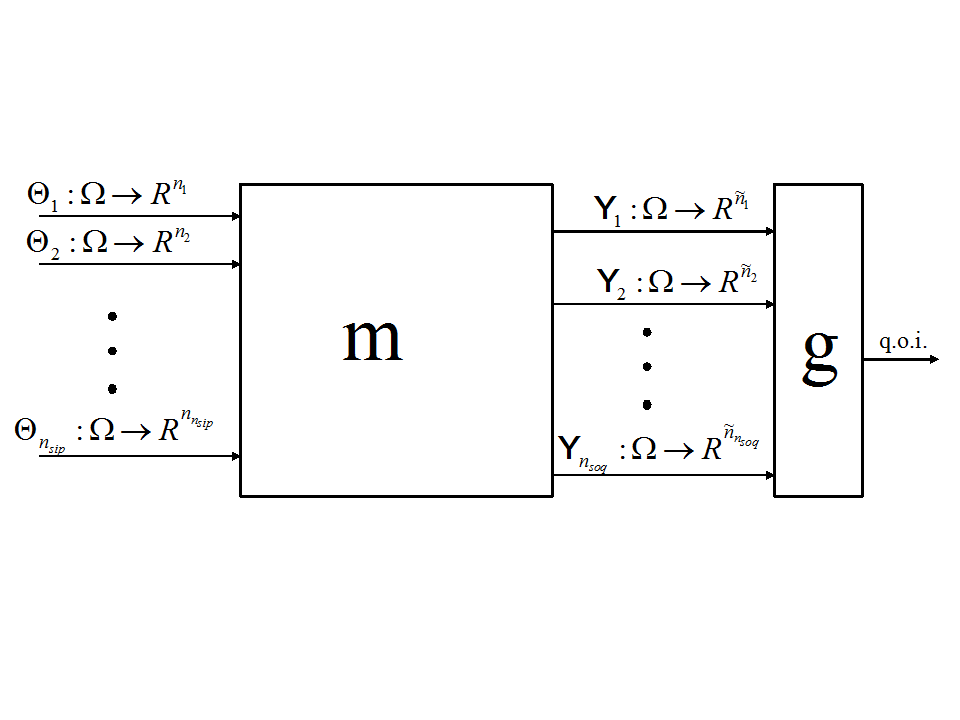
\includegraphics[scale=0.50,clip=true,viewport=0.1in 3.00in 13.1in 8.0in]{black_box3.eps}
\end{center}
\caption{A generic ``black-box'' system description.
}
\label{fig-black-box}
\end{figure}

However, we will assume that we do not have a detailed quantitative description of the distributions of the input parameters, so that we will need to solve a statistical inverse problem
in order to obtain such distributions, before propagating them through $m(\cdot)$ and $g(\cdot)$.
We will then suppose that
\begin{itemize}
\item there are $n_{\text{soq}}$ observations $\mathbf{y}_{j,\text{obs}}\in\mathbb{R}^{{\tilde{n}}_j}$, one for each of the output quantities,
\end{itemize}
and use the notations
\begin{eqnarray*}
\mathbf{y}_{\text{obs}} & = & (\mathbf{y}_{1,\text{obs}}\ldots,\mathbf{y}_{n_{\text{soq}},\text{obs}}), \\
R_{\text{sip}}          & = & \text{input subset of }\mathbb{R}^{N_{\text{sip}}}\text{ used for model exploration}.
\end{eqnarray*}

In order to be able to solve the statistical inverse problem, we will make the hypothesis that
\begin{equation}\label{eq-hyp-jpd}
\text{the joint probability density }\pi_{\boldsymbol{\Theta}\mathbf{Y}}:\mathbb{R}^{N_{\text{sip}}}\times\mathbb{R}^{N_{\text{soq}}}\rightarrow\mathbb{R}\text{ exists},
\end{equation}
\begin{equation}\label{eq-hyp-obs-mp}
\text{the marginal probability density }\pi_{m\mathbf{Y}}(\mathbf{y}_{\text{obs}})\neq 0,
\end{equation}
and
\begin{equation}\label{eq-hyp-theta-mp}
\text{the marginal probability density }\pi_{m\boldsymbol{\Theta}}(\boldsymbol{\theta})\neq 0\quad\forall\boldsymbol\theta\in R_{\text{sip}}.
\end{equation}
We emphasize that although we are assuming the existence of
$\pi_{\boldsymbol{\Theta}\mathbf{Y}}$ and
$\pi_{m\mathbf{Y}}(\mathbf{y}_{\text{obs}})$,
we will not need to know how to compute them.
Then,
\begin{equation*}
\text{the conditional probability }\pi_{\boldsymbol\Theta|\mathbf{y}}(\boldsymbol\theta|\mathbf{y}_{\text{obs}})\text{ exists }\forall\boldsymbol\theta\in\mathbb{R}^{N_{\text{sip}}}
\end{equation*}
and
\begin{equation*}
\text{the conditional probability }\pi_{\mathbf{Y}|\boldsymbol\theta}(\mathbf{y}_{\text{obs}}|\boldsymbol\theta)\text{ exists }\forall\boldsymbol\theta\in R_{\text{sip}},
\end{equation*}
that is, by Bayes theorem \eqref{eq-Bayes-2} we can claim that
\begin{equation*}
\pi_{\boldsymbol\Theta|\mathbf{y}}(\boldsymbol\theta|\mathbf{y}_{\text{obs}})
=
\frac
{\pi_{m\boldsymbol{\Theta}}(\boldsymbol{\theta})~\pi_{\mathbf{Y}|\boldsymbol\theta}(\mathbf{y}_{\text{obs}}|\boldsymbol\theta)}
{\pi_{m\mathbf{Y}}(\mathbf{y}_{\text{obs}})}
\quad\forall\boldsymbol\theta\in R_{\text{sip}}.
\end{equation*}
This last equation defines the solution of the statistical inverse problem. In the literature terminology it is written as
\begin{equation}\label{eq-sol-sip}
\pi_{posterior}(\boldsymbol\theta)
=
\frac
{\pi_{prior}(\boldsymbol{\theta})~\ell(\mathbf{y}_{\text{obs}}|\boldsymbol\theta)}
{\pi_{m\mathbf{Y}}(\mathbf{y}_{\text{obs}})},
\end{equation}
where $\ell(\cdot|\cdot)$ stands for ``likelihood''.
However, although we can claim the existence of the solution of the statistical inverse problem,
we are still not able to compute it, since the terms on the r.h.s. in \eqref{eq-sol-sip} are not yet known.
We then assume that
\begin{equation}\label{eq-hyp-prior-known}
\text{the prior probability density }\pi_{prior}(\boldsymbol{\theta}),~\boldsymbol\theta\in R_{\text{sip}},\text{ is known},
\end{equation}
\begin{equation}\label{eq-hyp-conditional-independence}
\text{the r.v.'s }\mathbf{Y}_j,~j=1,\ldots,n_{\text{soq}},\text{ are conditionally independent w.r.t. }\boldsymbol\theta,\quad\forall\boldsymbol\theta\in R_{\text{sip}},
\end{equation}
and
\begin{equation}\label{eq-hyp-l-known}
\text{each individual likelihood }\ell_j(y_{j,\text{obs}}|\boldsymbol\theta),~j=1,\ldots,n_{\text{soq}},~\boldsymbol\theta\in R_{\text{sip}},\text{ is known}.
\end{equation}
Although we cannot compute $\pi_{posterior}(\boldsymbol\theta)$,
since we do not have $\pi_{m\mathbf{Y}}(\mathbf{y}_{\text{obs}})$,
we can at least compute the quantity
\begin{equation}\label{eq-posterior-up2a-constant}
\tilde{\pi}(\boldsymbol\theta) =
{\pi_{prior}(\boldsymbol\theta)\prod_{j=1}^{n_{\text{soq}}}\ell_j(y_{j,\text{obs}}|\boldsymbol\theta)},
\end{equation}
that is, we can at least compute the posterior joint probability density function up to a multiplicative constant.
The importance of such computation is that there exist
appropriate chain generation methods that are proved to have their limiting distributions equal 
to the target distribution $\pi_{posterior}(\boldsymbol\theta)$ as long as the target distribution is supplied
up to a multiplicative constant, such as \eqref{eq-posterior-up2a-constant}, for instance.
The generation of such chains is precisely at the heart of the so called Markov Chain Monte Carlo (MCMC) methods
an is further discussed in Chapter \ref{ch-mcmc}.

Once a chain
\begin{equation}\label{eq-markov-chain-1}
\{\boldsymbol{\theta}^{(0)},\boldsymbol{\theta}^{(1)},\ldots\}
\end{equation}
is (approximately) generated according to $\pi_{posterior}(\boldsymbol\theta)$ using $\tilde{\pi}(\boldsymbol\theta)$,
one can
sample parameters from the chain,
run the simulation of the system for each selected sample and
collect statistical information for any desired quantities of interest.

\section{A More Detailed System Description}\label{sc-intro-detail}

The generic ``black-box'' system description of Section \ref{sc-intro-qoi} is flexible enough to model many different situations. Indeed, the system might:
\begin{itemize}
\item be at steady-state regime, or evolve with time, from instant $t=0$ until instant $t=T$,
\item be a physical system over a bounded physical domain $D\subset\mathbb{R}^3$,
\item need $n_{s}$ stochastic state variables $S_i$ for its description, $1\leqslant i\leqslant n_s$, and
\item have equations dictating how the domain and/or the values of the parameters and/or the state values vary with time $t$ and/or space position $\mathbf{x}\in D$.
\end{itemize}
We will denote
\begin{equation*}
\mathbf{S} = (S_1,\ldots,S_{n_s}).
\end{equation*}

\begin{figure}%[h]
\begin{center}
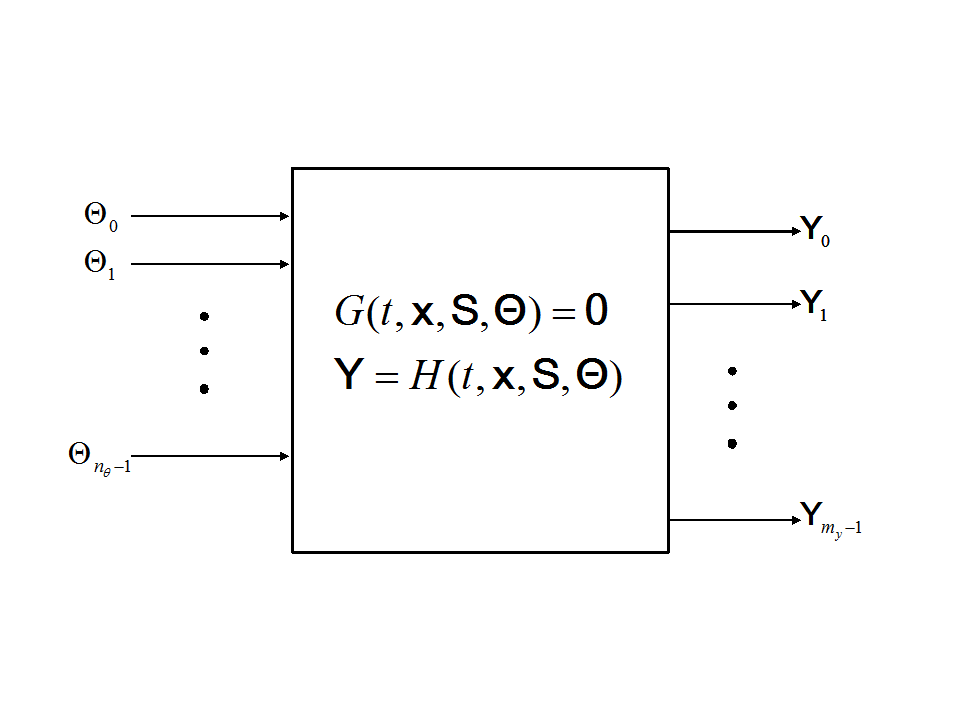
\includegraphics[scale=0.50,clip=true,viewport=0.8in 2.25in 12.0in 8.0in]{black_state.eps}
\end{center}
\caption{Generic model of a system with state $\mathbf{S}(t,\mathbf{x}) = (S_1(t,\mathbf{x}),\ldots,S_{n_s}(t,\mathbf{x}))$
evolving from instant $t=0$ until instant $t=T$
over positions $\mathbf{x}\in D\subset\mathbb{R}^3$.
}
\label{fig-state-model}
\end{figure}
